%11/10 - Luis del Peso
\chapter{Alineamiento de múltiples secuencias (MSA)}
¿Cuál es la ventaja del MSA frente a los alineamientos por pares? La principal ventaja es que hay mucha más información en un MSA que en un alineamiento por pares, por lo que al realizar un MSA mejoramos la relación señal/ruido. Consideremos el ejemplo de juguete de la figura \ref{fig:msa}. Muestra la alineación de un fragmento del dominio Ser/Thr-quinasa del AK77 humano con dos proteínas de archaea. Ambas alineaciones por pares son relativamente similares, por lo que sería difícil decidir cuál de ellas, si es que hay alguna, representa un verdadero homólogo de la consulta (los valores E son $3 \cdot 10^6$ y $7 \cdot 10^7$ respectivamente). Además, incluso sabiendo que el segundo alineamiento corresponde a un verdadero homólogo, sería difícil identificar qué residuos son esenciales para la actividad y/o el plegamiento del dominio quinasa. Sin embargo, un MSA de miembros de la familia Ser/Thr-quinasa revela los residuos clave del dominio catalítico. Además, esta información indica que el primer alineamiento corresponde a un falso positivo. Esto significa que, a pesar del valor E relativamente bajo, es poco probable que las proteínas alineadas compartieran un ancestro común. Este ejemplo también muestra que el MSA de un grupo de secuencias homólogas define los dominios o motivos que caracterizan a una familia de proteínas. Los residuos alineados en un MSA se derivan presumiblemente de un ancestro común, es decir, son homólogos en un sentido evolutivo. En consecuencia, los residuos conservados en un MSA tienden a ocupar posiciones correspondientes en la estructura tridimensional de cada una de las proteínas homólogas. Es importante señalar que las estructuras tienden a estar más conservadas que las secuencias dentro de una familia de proteínas. Así, para dos proteínas homólogas distantes, la conservación a nivel de residuos podría ser baja, por ejemplo un 30\% de identidad, mientras que tienen una proporción mucho mayor de residuos, por ejemplo un 50\%, localizados en posiciones equivalentes de sus estructuras tridimensionales. En consecuencia, los verdaderos homólogos distantes suelen tener una función bioquímica/biológica similar a pesar de la baja identidad de secuencia. Y lo que es más importante, utilizando MSA podríamos alinear dos secuencias distantes a través de su relación con una tercera secuencia, integrando así información no disponible en alineaciones por pares. Por ejemplo, si las proteínas A y C son homólogas muy distantes, un MSA que incluya una proteína B, relacionada tanto con A como con C, podría ayudar a construir el alineamiento correcto si B es equidistante a A y B en distancia evolutiva.

\begin{figure}[htbp]
\centering
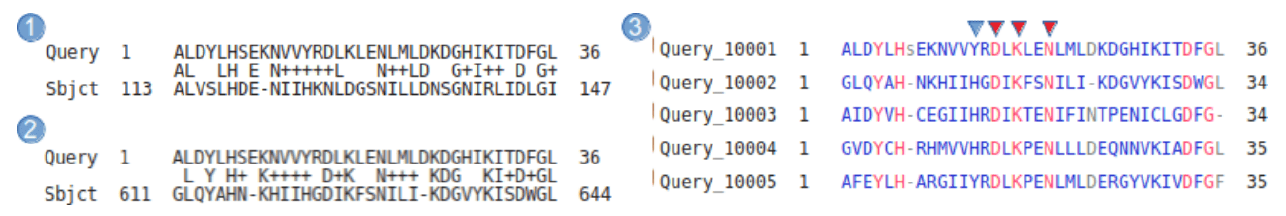
\includegraphics[width = \textwidth]{figs/msa.png}
\caption{\textbf{Pairwise vs MSA}. Se utilizó un fragmento del dominio quinasa de AKT7 humano (P31749) como consulta para buscar en una base de datos de proteínas archaca. (1) Alineación de AKTI y una ATPasa de la familia AAA (WP\_109940497.1) de \textit{Methanospirillum stamsii}. (2) Alineamiento del mismo fragmento de AKTI con una serina/treonina-proteína quinasa (OPY23844) de \textit{Methanobacterium sp}.. (3) MSA del sitio activo de 5 serina-treonina quinasas distantes. En flecha roja los residuos conservados en las 5 secuencias alineadas. Las puntas de flecha rojas marcan tres posiciones invariantes conservadas en todas las Ser/Thr-cinasas conocidas, el residuo Asp (D en esta tríada es el residuo del sitio activo. La punta de flecha azul marca una posición que está ocupada por His o Tyr en todas las proteínas conocidas de esta superfamilia).}
\label{fig:msa}
\end{figure}

\section{Métodos y esquemas de puntuación para la alineación de secuencias múltiples}
Como se explica en el capítulo anterior, la alineación óptima por pares puede lograrse eficazmente mediante algoritmos de programación dinámica. Estos métodos se basan en la construcción de una matriz $n \cdot m$, donde n y m corresponden a la longitud de las secuencias alineadas, y su complejidad en tiempo de ejecución es del orden de $O(n \cdot m)$ u $O(n^2)$ suponiendo que $n \sim m$. La extensión de este método a MSA es trivial. Por ejemplo, para tres secuencias de longitudes n, m y k, construiríamos una matriz $n \cdot m \cdot k$ que contenga las puntuaciones parciales óptimas para el alineamiento de tres posiciones. Sin embargo, la complejidad temporal en este caso sería de $O(n \cdot m \cdot k)$ u $O(n^3)$ suponiendo que $n \sim m \sim k$. De forma más general, para s secuencias de longitud n, la complejidad temporal sería $O(n^s)$ que crece exponencialmente con el número de secuencias. Por lo tanto, aunque este enfoque conduciría a un MSA óptimo, es poco práctico para más de unas pocas secuencias. Por este motivo, los métodos «simultáneos» no pueden aplicarse a problemas reales de MSA y se aproximan mediante métodos heurísticos que reducen el tiempo de cálculo pero no garantizan encontrar el alineamiento múltiple óptimo. Uno de los programas más populares para realizar MSA es ClustalW. Es un ejemplo de una familia de algoritmos que siguen una estrategia progresiva o jerárquica. Los métodos progresivos funcionan en tres pasos (véase la figura \ref{fig:clustalw}):
\begin{enumerate}
\item En el primer paso, este programa computa todos los posibles alineamientos por pares y calcula una puntuación bruta para cada alineamiento. La puntuación puede ser simplemente el porcentaje de identidades o medidas más sofisticadas.
\item A continuación, se realiza un análisis jerárquico de conglomerados en la tabla de puntuaciones por pares del paso anterior. Esta técnica produce un árbol guía o dendrograma que agrupa las secuencias según su similitud.
\item Por último, las secuencias se alinean progresivamente siguiendo la topología del árbol generado en el paso anterior. Así, se alinean las dos secuencias con la puntuación de similitud más alta y, a continuación, la secuencia siguiente se añade al alineamiento por pares o se utiliza en otro alineamiento por pares. Aunque no entraremos en detalles aquí, existen métodos rigurosos para alinear una secuencia contra un alineamiento. Imaginemos que la secuencia se alinea con una secuencia consenso derivada del alineamiento. El MSA puede representarse mediante estructuras matemáticas denominadas perfiles. En algún momento, los perfiles se alinean con los perfiles. Por último, el MSA se genera siguiendo el árbol guía desde los nodos más terminales hasta la raíz.
\end{enumerate}

\begin{figure}[htbp]
\centering
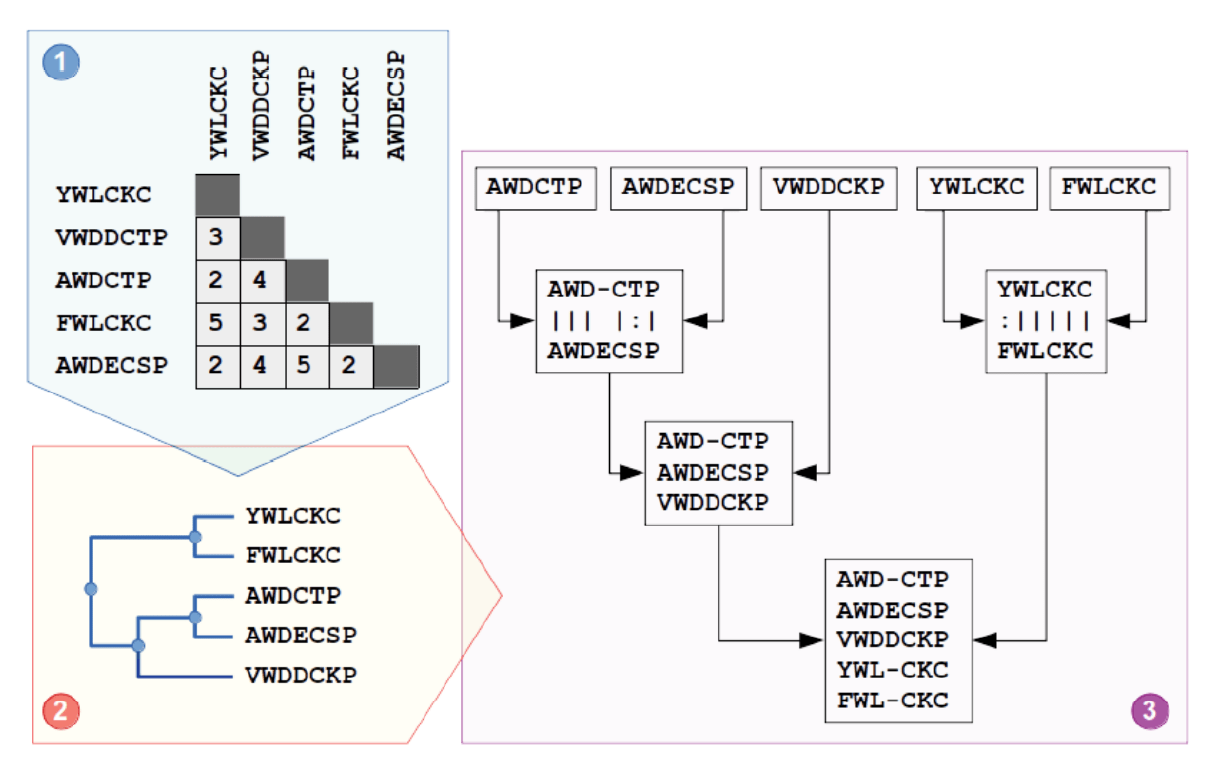
\includegraphics[width = \textwidth]{figs/clustalw.png}
\caption{\textbf{Métodos progresivos para el MSA}. Para producir un MSA de las secuencias YWLCKC (secuencia A), VWDDCTP (secuencia B). AWDCTP (secuencia C), FWLCKC (secuencia D) y AWDECSP (secuencia E), los métodos progresivos comparan primero todos los pares de secuencias (no mostrados) y registran la puntuación de cada alineamiento por pares (1). A continuación, basándose en estas puntuaciones, el algoritmo produce un árbol guía (2). Por último, las secuencias se alinean progresivamente empezando por las más cercanas. En cada paso del proceso, el algoritmo sigue la topología del árbol desde las hojas hasta la raíz, añadiendo nuevas secuencias o alineaciones en cada nodo del árbol (3).}
\label{fig:clustalw}
\end{figure}

Además de ClustalW, otras herramientas implementan variaciones de este algoritmo progresivo. Por ejemplo, ClustalW utiliza programación dinámica para el alineamiento por pares inicial, que es preciso pero puede ser lento para un gran número de secuencias. Por esta razón, otros métodos, como Kalign, cuentan el número de k-mers compartidos por las secuencias para calcular la distancia entre todos los pares. La ventaja de este método es que no es necesario alinear las secuencias para generar la matriz de distancias.

Uno de los problemas de los métodos progresivos es que el orden en que se añaden gradualmente las secuencias puede tener un fuerte impacto en el MSA final. Además, cuando se produce un error en un alineamiento intermedio, suele propagarse en los alineamientos posteriores. Esto es especialmente cierto en el caso de los gaps. Para mitigar estos problemas, diferentes algoritmos han adoptado variaciones en el procedimiento general, pero no las discutiremos aquí. Otro problema no resuelto en MSA es cómo calcular la puntuación. Se han propuesto varias estrategias:
\begin{itemize}
\item Scoring basado en una secuencia de referencia: $S_{MSA} = S_{AB} + S_{AC} + S_{AD} + S_{AE} $
\item Scoring basado en el dendograma: $S_{MSA} = S_{AB} + S_{CD} + S_{CD/E} + S_{AB/CDE}$
\item Scoring basado en la suma de alineamientos por pares: $S_{MSA} = S_{AB} + S_{AC} + S_{AD} + S_{AE} + S_{BC} + S_{BD} + S_{BE} + S_{CD} + S_{CE} + S_{DE}$
\end{itemize}

En resumen, aún no se ha resuelto el problema de calcular un MSA óptimo en un tiempo práctico. Mientras tanto, se han desarrollado varios enfoques heurísticos para calcular soluciones aproximadas que no garantizan ser la mejor solución posible.

Hasta ahora nos hemos centrado en el MSA de proteínas, sin embargo, el alineamiento múltiple de secuencias de regiones genómicas merece especial atención debido a la creciente cantidad de genomas completos disponibles y a su relevancia para identificar regiones genómicas reguladoras y comprender la variabilidad genética interindividual e interespecífica. Aunque no entraremos en detalles, la alineación de regiones genómicas plantea retos específicos. Por ejemplo, los genomas contienen un gran número de regiones repetitivas que son difíciles de alinear con precisión. Además, aunque la secuencia de determinadas regiones del genoma pueda conservarse en diferentes especies, a menudo la posición relativa de las distintas porciones del genoma no se conserva debido a reordenamientos genómicos. Por último, los MSA proteínicos suelen estar formados por un gran número de secuencias relativamente cortas, mientras que ocurre lo contrario con los MSA genómicos. Por todas estas razones, la alineación genómica requiere métodos de MSA especializados. Uno de ellos es MLAGAN, que se basa en un método progresivo similar al utilizado por ClustalW, y MULTIZ, utilizado para producir el MSA genómico que muestra el navegador del genoma de la UCSC.

\subsection{Ejemplo: FOXP2}
FOXP2 es un factor de transcripción. Al realizar un alineamiento de múltiples secuencias, se observan algunos residuos que presentan unos cambios únicos en humanos y son los que nos aportan la capacidad de comunicación como el habla. Además, individuos que tienen mutados esos individuos presentan un desorden del lenguaje. Por tanto, esos residuos son clave, y esto se demostró en ratones a los que se les cambió esos residuos concretos. Visto que esos cambios aparecen específicamente en humanos y que introducidos en ratones producen un comportamiento similar al habla, se analizó la filogenia y se observó exclusivamente en \textit{Homo sapiens} y Neandertales, pero no en otros primates.

\begin{figure}[htbp]
\centering
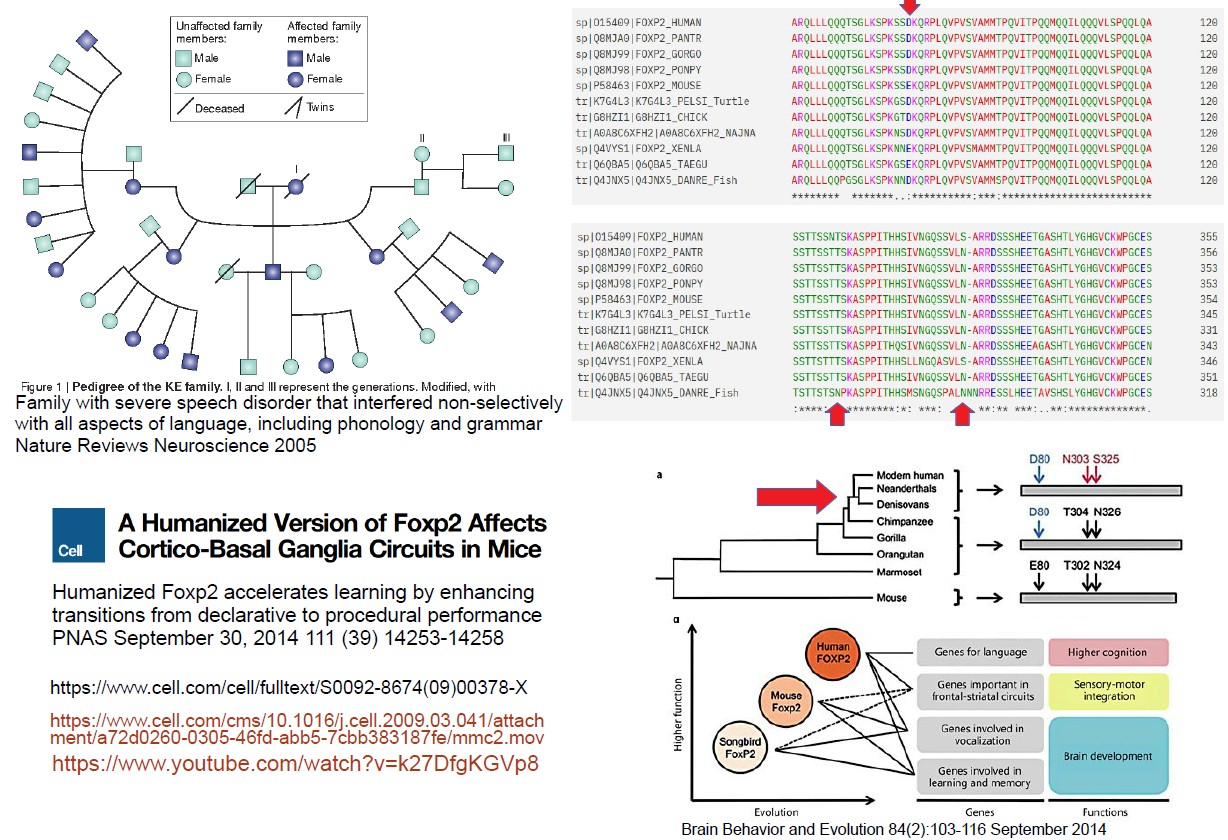
\includegraphics[width = \textwidth]{figs/foxp2.png}
\caption{Ejemplo del factor de transcripción FOXP2}
\end{figure}

%14/10 - Luis del Peso
\section{Representación de MSA}
Como se ha explicado anteriormente, el MSA puede utilizarse para identificar motivos/dominios funcionales y/o estructurales en un grupo de secuencias. Y lo que es más importante, una vez que hemos identificado ese motivo/dominio, puede utilizarse para buscar en bases de datos e identificar otras proteínas que compartan ese (nuevo) motivo y, como veremos, esas búsquedas son mucho más sensibles que las basadas en una secuencia de consulta. Sin embargo, para realizar dichas búsquedas, necesitamos una forma de representar el motivo/dominio revelado en el MSA. Existen varias formas de representar una región conservada, como se explica a continuación.

\subsection{Secuencia consenso}
Esta es la forma más sencilla de representar una región conservada y se utiliza ampliamente debido a su simplicidad y a su interpretación directa. Para construir una secuencia de consenso podríamos limitarnos a representar aquellos residuos que se conservan en todas las secuencias en una posición determinada. Por ejemplo, la secuencia consenso para la MSA representada en la figura \ref{fig:consensus-seq} es: TTxCxxAAxx donde x representa cualquier aminoácido. De hecho, esto se denomina consenso al 100\% de frecuencia, porque un residuo sólo se incluye en el consenso cuando está presente en el 100\% de las secuencias alineadas. El consenso puede construirse a cualquier otro nivel de porcentaje. Para el mismo alineamiento, el consenso al 50\%, que representa residuos presentes en al menos el 50\% de las secuencias, sería TTGCTCAAXT. Por último, a menudo el consenso representa el residuo más frecuente en cada posición, independientemente de su frecuencia absoluta.

\begin{figure}[htbp]
\centering
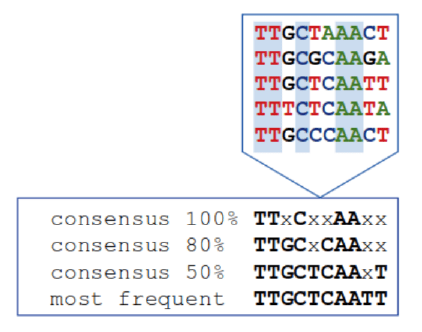
\includegraphics[width = 0.5\textwidth]{figs/consensus-seq.png}
\caption{\textbf{Secuencia consenso.} La secuencia de consenso indica el residuo presente en al menos un determinado porcentaje de las secuencias alineadas, o simplemente el residuo más frecuente, en cada posición del MSA. La figura muestra la alineación de varias secuencias de ADN unidas por C/EBP.}
\label{fig:consensus-seq}
\end{figure}

\subsection{Expresiones regulares o patrones}
El problema de las secuencias de consenso es que se pierde la mayor parte de la información contenida en el alineamiento. Por ejemplo, el consenso TTxCxxAAxx implica que no hay preferencia de residuo en la tercera posición. Sin embargo, la inspección de las secuencias individuales revela que, de hecho, existe una fuerte preferencia por la guanina en esta posición.
Por otra parte, el consenso del 50\% capta la preferencia por G en esta posición, pero no informa sobre qué otros residuos (si los hay) pueden ocupar esta posición ni sobre su frecuencia. Esta deficiencia es evidente en la décima posición del consenso del 50\%, que no muestra que en esta posición son posibles tanto la timina como la adenina. Las \textbf{expresiones regulares}, también conocidas como \textbf{patrones}, utilizan un conjunto de reglas para capturar esta diversidad. Por ejemplo, representan todos los residuos alternativos posibles en una posición determinada entre corchetes. También se puede representar aquellos residuos que nunca aparecen entre llaves. Así, el MSA de la figura \ref{fig:consensus-seq} puede representarse mediante la expresión regular:\\
TT[GT]C[TGC][AC]AA[TGC][TA]\\
TT[GT]C\{A\}[AC]AA\{A\}[TA]\\
Esta representación proporciona más información que las contras correspondientes, ya que muestra que la décima posición puede estar ocupada por T o A.

\subsection{Matrices de puntuación específicas para cada puesto (PSSM)}
Aunque las expresiones regulares representan una mejora con respecto al consenso, pierden importante información orientativa. La expresión regular mostrada en la sección anterior indica que T, C o G pueden encontrarse en las posiciones quinta y novena. Sin embargo, la preferencia por la timina es mayor en la quinta posición (0,6 frente a 0,4 de frecuencia). Una estructura que captura este tipo de información cuantitativa es la Matriz de Puntuación de Posiciones Específicas (PSSM). Una PSSM no es más que una matriz que confronta todos los símbolos posibles (los 20 aminoácidos posibles o los 4 nucleótidos en las secuencias de nucleótidos) con las posiciones de alineación. Cada celda de la matriz contiene un número que representa la preferencia de cada residuo concreto en cada posición. Hasta ahí, se consideraría una PWM (position weight matrix), es decir, tomar las frecuencias de cada nucleótido para cada posición normalizadas. Formalmente, los valores de cada celda de la PSSM se calculan como la relación logarítmica entre las frecuencias de residuos observadas en cada posición y las esperadas por azar. Así, suponiendo frecuencias de fondo iguales para todos los nucleótidos, el PSSM que representa el MSA mostrado en \ref{fig:consensus-seq} sería:

\begin{table}[htbp]
\centering
\begin{tabular}{l | l l l l l l l l l l }
& 1 & 2 & 3 & 4 & 5 & 6 & 7 & 8 & 9 & 10 \\ \hline
A & -1,2 & -1,2 & -1,2 & -1,2 & -1,2 & 0 & 1,4 & 1,4 & -1,2 & 0,4 \\
C & -1,2 & -1,2 & -1,2 & 1,4 & -0,2 & 1,2 & 1,2 & 1,2 & 0,4 & -1,2  \\
G & -1,2 & -1,2 & 1,2 & -1,2 & -0,2 & -1,2 & -1,2 & -1,2 & -0,2 & -1,2  \\
T & 1,4 & 1,4 & -0,2 & -1,2 & 0,8 & -1,2 & -1,2 & -1,2 & 0,4 & 0,8  \\
\end{tabular}
\caption{PSSM representando el MSA de la figura \ref{fig:consensus-seq}}
\end{table}

Por ejemplo, la entrada correspondiente a la timina en la posición 1 se calcularía como $log_2 \frac{5/5}{0,25} = 1,4$. Sin embargo, como $log_2(0)$ no está definido, esta ecuación produciría un error si se aplicara a la entrada de A en la primera posición $(log_2(\frac{0/5}{0,25}))$. Para evitar este problema utilizamos \textbf{pseudoconteos}, es decir, añadimos un pequeño valor, $\beta$, a cada celda para que la frecuencia observada nunca sea cero. Así, si la frecuencia observada del símbolo $i$ en la posición $p, f_{ip}$ es $n_{ip}/N_{seq}$, donde $n_{i,p}$ es el número de residuos del tipo $i$ alineados en la columna $p$ y $N_{seq}$ es el número de secuencias alineadas, entonces la frecuencia de $i$ después de añadir pseudoconteos sería:
$$f_{i,p} = \frac{n_{i,p} + \beta}{N_{seq} + (\beta \cdot N_s)}$$

donde $N_s$ es el número de los diferentes símbolos (4 en el caso de los nucleótidos y 20 para proteínas). Obsérvese que, de hecho, esta corrección es una forma de superar la falta de datos a la hora de derivar los valores de un PSSM. Por ejemplo, en el caso de la figura \ref{fig:consensus-seq}, ¿hasta qué punto estamos seguros de que la adenina nunca se encuentra en la posición 1? Si en lugar de sólo cinco instancias de C/EBP tuviéramos 500, ¿tendrían algunas de ellas «A» en la primera columna? El valor de $\beta$ suele ser 1 para la construcción de PSSMs, lo que implica que observaríamos al menos un residuo de cada tipo en cada columna si tuviéramos datos suficientes, pero podríamos elegir cualquier otro valor. Tras aplicar pseudoconteos la entrada correspondiente a la timina en la posición 1 se calcularía como $log _2(\frac{6/9}{0,25}) = 1,41$ y la entrada de A en la primera posición sería $log_2(\frac{1/9}{0,25}) =-1,2$.

El problema de este modelo es que asume la independencia entre posiciones, cuando esto es falso. Además, no se pueden representar fácilmente los gaps, solo se podría apañar haciendo una PSSM antes del gap y otra después.

\subsubsection{Generación de PSSM: un caso real}
En el siguiente ejemplo se oberva la frecuencia de nucleótidos en el motivo TATA derivado de más de 800 secuencias de promotores de mamíferos de GenBank que tenían anotados un motivo TATA.

\begin{figure}[htbp]
\centering
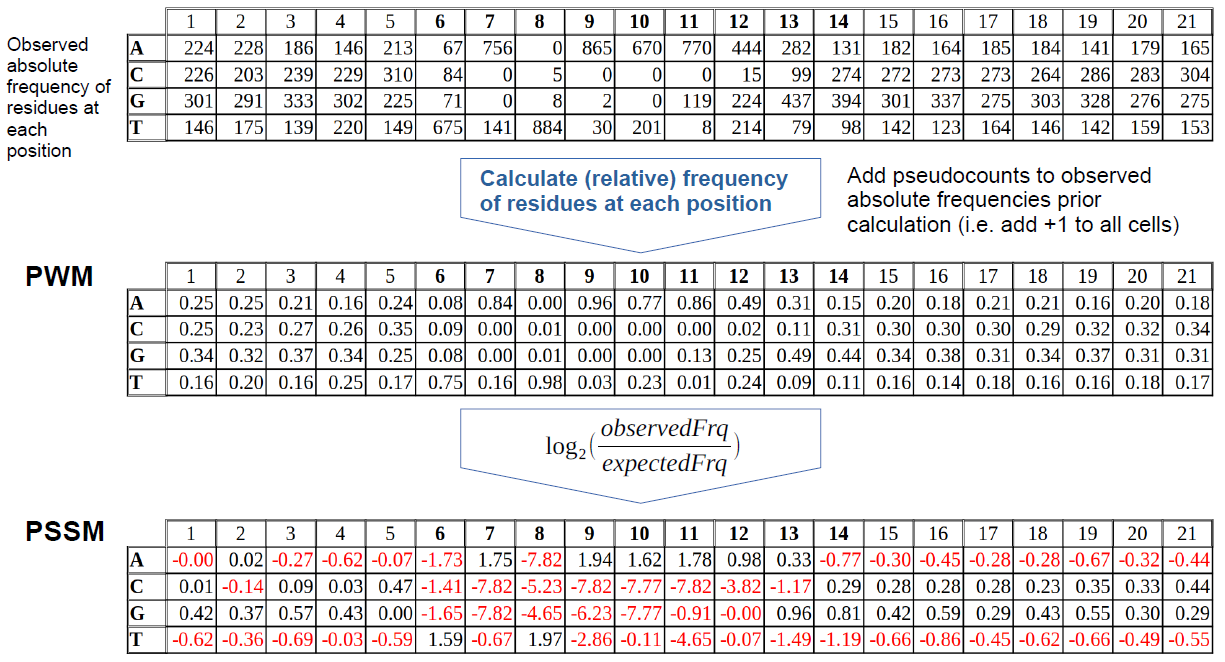
\includegraphics[width = \textwidth]{figs/tata.png}
\caption{Frecuencia de nucleótidos en el motivo TATA derivada de >800 secuencias promotoras de mamíferos de GenBank que tenían elementos TATA anotados a $\sim$ -30 pb del TSS.}
\end{figure}

\subsection{Secuencia de logotipos y contenido informativo}
Los PSSM y los HMM son formas precisas de representar la MSA. Son especialmente fáciles de manipular por ordenador y, por tanto, aptos para representar motivos y dominios proteicos en bases de datos especializadas y para buscar en bases de datos. Sin embargo, no son una forma fácil de representar MSA para el ser humano.

Por este motivo, en publicaciones y libros, los patrones de un conjunto de secuencias alineadas se suelen mostrar mediante una representación gráfica denominada \textbf{logo}. En un logo, los símbolos encontrados en cada posición del alineamiento se muestran apilados unos sobre otros, ordenados según su frecuencia (el símbolo más frecuente se muestra encima del resto). Además, la altura de los símbolos es proporcional a su frecuencia, de modo que se resaltan los símbolos preferidos en cada posición. Por último, la altura total de cada columna de símbolos se ajusta para significar la conservación global de los símbolos. Así, las posiciones que muestren una fuerte preferencia por un determinado tipo de residuos serán altas, mientras que las posiciones que muestren poca conservación estarán representadas por una pila corta de símbolos. La representación resultante revela claramente el patrón que definen las secuencias alineadas (véase la figura \ref{fig:logo}).

\begin{figure}[htbp]
\centering
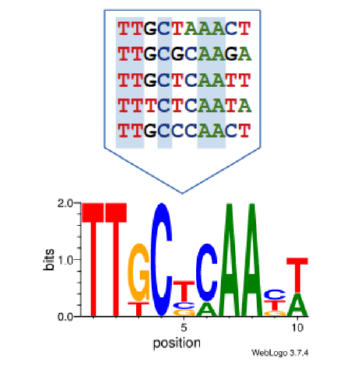
\includegraphics[width = 0.3\textwidth]{figs/logo.png}
\caption{\textbf{Logo}. Representación de la alineación mostrada en la figura \ref{fig:consensus-seq} como logo. El gráfico se generó con WebLogo3 sin ajustes de composición y utilizando un esquema de colores clásico.}
\label{fig:logo}
\end{figure}

Los logos de secuencias se basan en el concepto de entropía de la teoría de la información, desarrollado por Claude Shannon. El grado de conservación de los residuos en una posición concreta de un MSA puede cuantificarse, utilizando las herramientas de la teoría de la información, como la cantidad de incertidumbre sobre los posibles residuos que pueden ocupar esa posición. Por ejemplo, dado el MSA representado en la figura \ref{fig:logo}, nuestra incertidumbre sobre el nucleótido que puede encontrarse en la posición 1 de un sitio de unión a C/EBP es muy pequeña. Así, si alguien encuentra una nueva región unida por C/EBP será fácil predecir el nucleótido presente en la primera posición antes de ver este nuevo sitio de unión. En cambio, sería mucho más difícil predecir con certeza la identidad del residuo en la novena posición. En el campo de la información, la entropía \footnote{Formalmente, se llama entropía de Shannon}, H, de una variable aleatoria discreta X con valores posibles $x_1, x_2, \ldots ,x_n$ es una medida de la cantidad de incertidumbre asociada al valor de X (cuantifica la información). La entropía de Shannon se define como:
$$H(X) = -\sum_i P((x_i) log_2 P(x_i)$$
donde $P(x_i)$ es la probabilidad de observar el valor $i$-ésimo de X. La entropía, $H(X)$, se mide en unidades de bits. El término bit (que no byte) es una acortación de "binary digit" y representa la unidad básica de información en comunicación computacional y digital. En ese sentido, el término $P(x_i) log_2 P(x_i)$ es 0 cuando $P(x_i) = 0$.

Podemos pensar en los bits como el número mínimo de dígitos binarios necesarios para representar todos los estados de un sistema. Por ejemplo, el lanzamiento de una moneda puede dar dos resultados (estados): cara o cruz. Un solo dígito binario puede representar ambos (0 o 1). Por tanto, la entropía asociada al lanzamiento de una moneda es: $-(P_{head} log_2 P_{head} + P_{tail} log_2 P_{tail}) = 1 bit$. 
Del mismo modo, lanzar un dado puede dar lugar a 6 estados diferentes, por lo que para representar todos los casos posibles necesitaríamos tres dígitos binarios. Nótese que, en este caso, tres dígitos binarios es un exceso, ya que pueden representar hasta 8 estados (000, 001, 010, 100, 011, 101, 110, 111), mientras que nosotros sólo necesitamos representar 6. Sin embargo, dos dígitos binarios serían insuficientes para representar los seis estados. Por eso la entropía asociada es de 2,6 bits en lugar de 3. Último ejemplo: la incertidumbre de que haya un nucleótido en una cierta posición es:
\begin{align*}
H(nucleotide) = - \sum_{x_i = A, C, G, T} P(x_i) log_2 P(x_i) = \\
 - ((\frac{1}{4} \cdot log_2\frac{1}{4}) + (\frac{1}{4} \cdot log_2\frac{1}{4}) + (\frac{1}{4} \cdot log_2\frac{1}{4}) + (\frac{1}{4} \cdot log_2\frac{1}{4})) = 2 bits
\end{align*}
Por tanto, el genoma humano puede almacenar una capacidad máxima de información de:
$$3,2 \cdot 10^9 pb \cdot 2 bits = 6,4 \cdot 10^9 bits = 800 Mb = 0,8 Gb$$
Solo se tiene en cuenta una cadena y no las dos ya que, al ser complementarias, la información codificada es la misma en ambas cadenas y, por tanto, redundante. 
Bajo los estándares actuales, esta cantidad de información es ridícula. En el ADN está toda la información necesaria para hacer cualquier individuo completo. No obstante, el genoma codificante es un 1-2\%. Esto es crítico, ya que se genera mucha complejidad con tan poca información. El tema está en que nuestro genoma no codifica la información de cada neurona, solo codifica proteínas, las cuales interaccionan entre sí y generan propiedades emergentes. Así, hay una capa superpuesta de información que no es evidente y explica toda la complejidad. 
Nuestro genoma acumula muy poca información, pero es muy pequeño. Por unidad de volumen, la densidad de información a guardar es mucho más grande. Otra ventaja fundamental es que el ADN es muy estable, incluso almacenado de forma no óptima. Por ejemplo, los fósiles siguen teniendo ADN que se puede recuperar; no se puede decir lo mismo de un teléfono móvil 3 semanas a la intemperie. Por ello, se está intentando almacenar información en el ADN, pero el problema es cómo guardarlo y recuperarlo, ya que depende de procesos bioquímicos sensibles.

Volviendo a los logos, la altura de cada columna de símbolos representa el contenido informativo de esa posición concreta. Debemos pensar en el contenido informativo como una disminución de la incertidumbre tras la recepción de algún mensaje o dato. Así, el contenido informativo o entropía relativa es la diferencia entre la entropía (es decir, la incertidumbre) antes y después del mensaje:
$$I(X) = H_b(X) - H_a(X)$$
donde $I(X)$ es la información, $H_b$ la incertidumbre inicial y $H_a$ la entropía después de haber recibido algunos datos.
Por ejemplo, la incertidumbre sobre el resultado de tirar un dado antes de lanzarlo es de 2,6 bits. Si alguien tira los dados (sin que veamos el resultado) y nos informa de que el resultado ha sido un número par, entonces la entropía tras recibir este nuevo dato es de 1,6 bits. Así, podemos cuantificar la información recibida como $H_{before} - H_{after}$ correspondiente a 1 bit. En el caso de las secuencias biológicas, ver el MSA reduce nuestra incertidumbre sobre el símbolo esperado en cada posición y esta reducción se cuantifica por el contenido de información de cada posición. Nótese que hemos estado calculando el contenido de información para posiciones individuales. La ganancia total de información se obtiene sumando todas las posiciones. Al hacerlo, partimos del supuesto simplificador de que las frecuencias de una posición no se ven influidas por las de otra posición. Así, el contenido total de información para el MSA se calcula como:
$$I = \sum_i H_i^b - H_i^a$$
donde $i$ representa cada posición en el alineamiento.

\begin{table}[htbp]
\begin{mdframed}[backgroundcolor=black!10]
En resumen, los logos son representaciones de los alineamientos donde se representan los nucleótidos en cada posición, siendo el tamaño del nucleótido representativo de su frecuencia. En este caso, el eje y muestra bits, que son una unidad de información. Cuantas más posibilidades (outcome, $x_i$) hay, más incertidumbre hay y, por tanto, mayor es la entropía de Shannon. 

Algunas posiciones llegan a los 2 bits, es decir, almacenan toda la información que es posible almacenar. Sin embargo, hay otras posiciones que son menores que 2 bits. Esto se debe a que no se muestra la entropía, si no la información: la incertidumbre de un proceso antes y después de recibir información adicional. Antes de un alineamiento, la incertidumbre en cada posición es de 2 bits. Si tras hacer el alineamiento una posición tiene siempre un mismo nucleótido, la incertidumbre pasa a ser 0, por lo que la información es 2 - 0 = 2. Cuanto más variable sea una posición en el alineamiento, más incertidumbre hay y menos información tenemos. En los logos, la altura es el contenido de información y el tamaño de cada letra es la probabilidad de que salga.
\end{mdframed}
\end{table}

\begin{figure}[htbp]
\centering
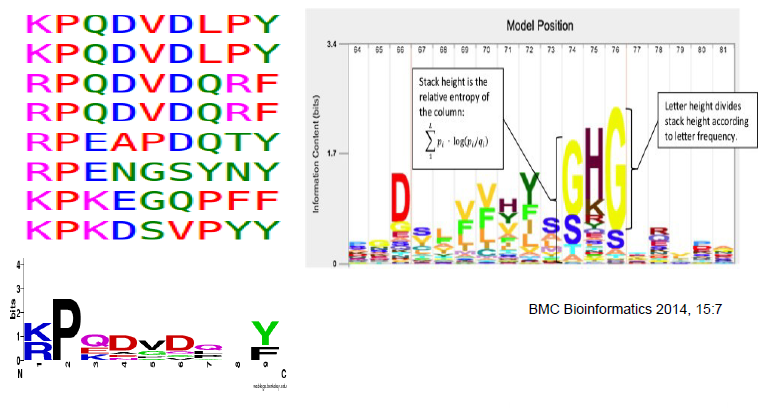
\includegraphics[width = 0.8\textwidth]{figs/logo-parts.png}
\caption{Partes de un logo.}
\end{figure}

%16/10 - Luis del Peso 
\subsection{Modelos de Markov ocultos (HMM)}
Aunque un PSSM es un modelo cuantitativo que capta la mayor parte de la información del MSA, presenta algunas limitaciones. En concreto, los PSSM no tienen en cuenta las deleciones ni las inserciones. Además, asume la independencia de las posiciones. Para superar esta limitación, podríamos tratar los gaps en el MSA combinando las puntuaciones de los subalineamientos sin gaps. De hecho, este es el enfoque adoptado en la base de datos BLOCKS.

Un enfoque más flexible y potente consiste en utilizar un modelo probabilístico denominado \textbf{Modelo de Markov Oculto (HMM)}. Los HMM son modelos probabilísticos que se desarrollaron para el reconocimiento del habla, pero ahora se utilizan ampliamente en muchos campos. En el caso de la bioinformática, los HMM se han utilizado en la segmentación\footnote{Las secuencias de ácidos nucleicos y proteínas pueden contener regiones distintas cuya composición de residuos y función biológica pueden diferir. Por ejemplo, el genoma puede segmentarse en regiones funcionales que incluyen, promotores, potenciadores, intros, exones, ... Los HMM pueden ayudarnos a definir los límites exactos de estas regiones.}, la búsqueda de genes y la alineación de secuencias, por nombrar algunos. La principal ventaja de los HMM en el análisis de secuencias es que se basan en un modelo probabilístico sólido y el modelo incluye una representación explícita de los INDEL (inserciones y deleciones, es decir, huecos). Los MSA también pueden representarse como HMM y los HMM que describen familias de secuencias relacionadas se denominan \textbf{HMM de perfil}.

\textbf{Ejemplo:}
En una secuencia, lo "visible" son los nucleótidos, mientras que la categoría invisible son las etiquetas de las regiones ricas en GC y ricas en AT. Dependiendo de la región en la que se encuentre un nucleótido, su frecuencia es diferente. Eso se recoge en la matriz de emisión: muestra la probabilidad de cada nucleótido en un estado concreto (probabilidad condicionada). Además, como se irá viendo la secuencia en dirección 5' a 3', llegará un momento de transición de una región a otra. La probabilidad de pasar de un estado a ese mismo (no cambiar de estado) o a otro estado se recoge en la matriz de transición.

\begin{figure}[htbp]
\centering
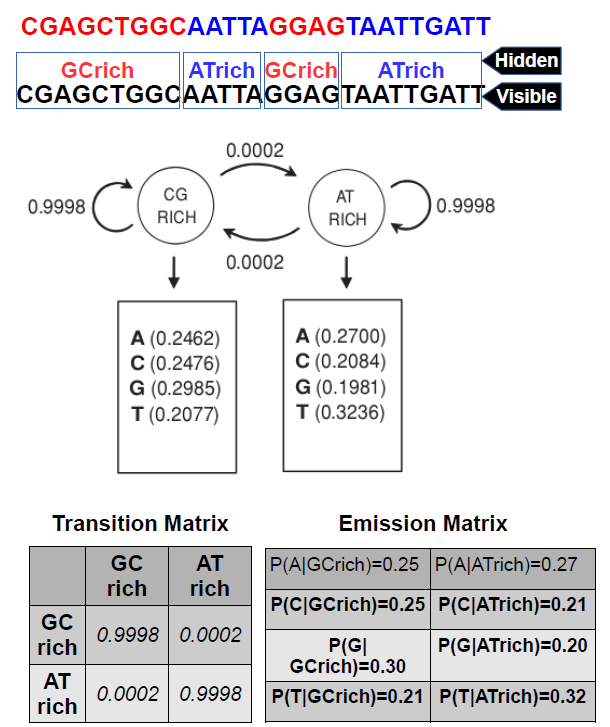
\includegraphics[width = 0.5\textwidth]{figs/transition-emission.png}
\caption{Ejemplo}
\end{figure}

%El estado match es aquella columna en la que tenga el símbolo al menos el 50% de las secuencias
En los \textbf{HMM de perfil}, los residuos de cada posición de la alineación pueden estar en uno de los \textbf{tres estados posibles: Match, Insert o Delete}. Los estados Match representan posiciones conservadas en el MSA (aunque no exclusivamente residuos similares), mientras que los estados Insert representan pequeños tramos de secuencia inespecífica. Los estados Delete corresponden a huecos y representan la ausencia de un residuo conservado (es decir, una posición Match) en uno o unos pocos miembros de la familia. Así, dado un MSA, las columnas que contienen sólo residuos alineados o residuos alineados en la mayoría de las secuencias se modelan como una posición de estado de coincidencia. Algunas de las secuencias pueden tener un hueco en una columna de coincidencia. Por otro lado, una columna en el alineamiento en la que la mayoría de las secuencias no tienen un residuo se considera una columna en estado de inserción. En términos prácticos, se considera que una columna está compuesta por inserciones cuando sólo una fracción específica de las secuencias (por ejemplo, menos del 50\% de las secuencias) muestran un residuo en esa columna en particular\footnote{Obsérvese que, en las columnas de inserción, las secuencias sin residuos no tienen hueco (que representa la ausencia de un residuo conservado), aunque normalmente se utiliza un guión («-», símbolo de hueco) para rellenar el espacio. De hecho, en algunos casos se utiliza un símbolo diferente (por ejemplo, un punto, para indicar la diferencia).}. Ambos estados, Match e Insert, tienen asociadas probabilidades de emisión que corresponden a las probabilidades de observar cada aminoácido en esa posición concreta del alineamiento. De forma similar a la construcción de PSSMs, cuando se produce un HMM a partir de un MSA, las probabilidades de emisión se derivan de las frecuencias observadas de residuos en cada columna M (coincidencia, match) o I (inserción, insert). Obviamente, los estados D (borrar, delete) no tienen probabilidades de emisión asociadas. Por ejemplo, en la alineación de la figura \ref{fig:prof-hmm} hay diez columnas de estado de coincidencia y una columna de inserción. Las frecuencias de los residuos en cada estado definen las \textbf{probabilidades de emisión} para ese estado. Además, la definición completa de un HMM requiere las \textbf{probabilidades de transición}. Estas probabilidades describen la frecuencia de observar una coincidencia, inserción o eliminación en la columna $i + 1$ dado el estado en la columna $i$. En el ejemplo de la figura \ref{fig:prof-hmm}, la probabilidad de transición de M1 a M2 es 1. Sin embargo, sólo 8 de las 10 secuencias van de M4 a M5 y las dos secuencias restantes tienen una inserción en la posición de nido (I4). Así, la probabilidad de transición de M4 a M5 es 0,8 y de M4 a I4 es 0,2. Obsérvese que la suma de las probabilidades de transición de un estado dado es igual a 1. Por último, los HMM incluyen dos estados denominados «inicio» y «fin» que no corresponden a ninguna columna del MSA y sólo se requieren para especificar todas las probabilidades de transición (se consideran estados «coincidentes»).

En resumen, para construir el gráfico de HMM (figura \ref{fig:prof-hmm}), primero se definen las posiciones match de los alineamientos. Para ello, tenemos en cuenta que al menos el 50\% de las secuencias tengan el mismo residuo en una determinada posición. Ese valor lo hemos utilizado para el ejemplo en clase, pero en realidad está muy calculado y calibrado. Una vez definidas estas posiciones, se buscan los residuos que estén en estado de inserción o deleción. Los estados de deleción se refieren a símbolos o residuos concretos que se encuentran en una posición que está en match. En el caso de los estados de inserción, alguna secuencia presenta en una posición un residuo, pero esa posición no está presente en la mayoría de las secuencias y, por tanto, no está en match. Para diferenciar los estados de inserción y deleción en un alineamiento, se pueden utilizar los guiones para las deleciones y puntos para las posiciones que no presentan la inserción. Cada secuencia concreta sigue un camino en el gráfico. 

\begin{figure}[htbp]
\centering
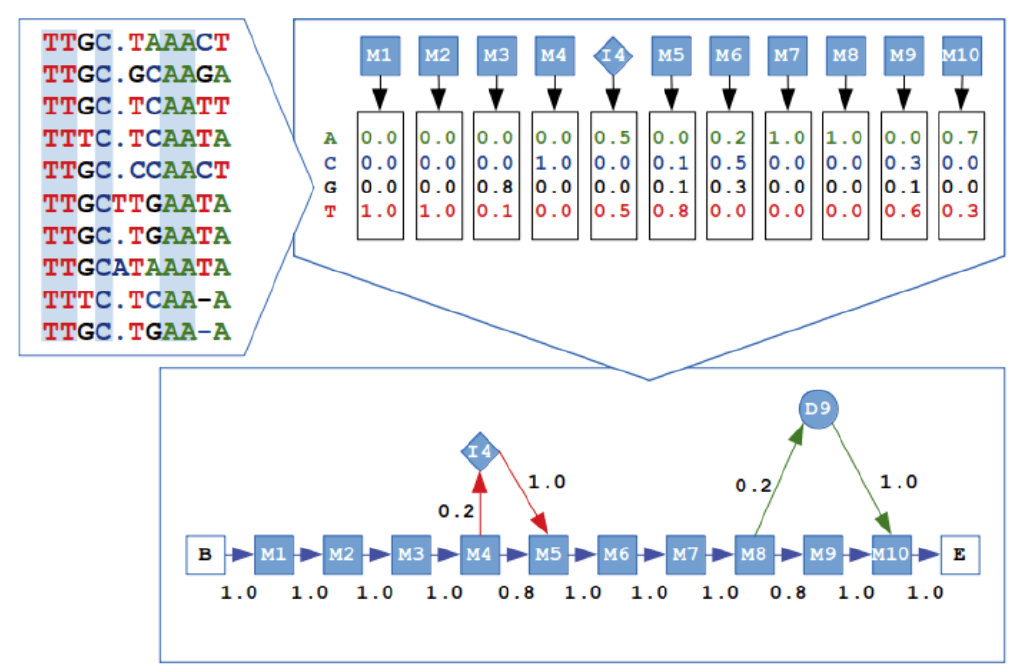
\includegraphics[width = 0.7\textwidth]{figs/profile-hmm.png}
\caption{\textbf{HMM de perfil}. Representación del alineamiento mostrado en la figura \ref{fig:consensus-seq} como un HMM de perfil. Nótese que se han añadido tres secuencias adicionales, incluyendo una secuencia con una inserción y dos secuencias con una deleción (las dos últimas secuencias). El panel de la izquierda del alineamiento muestra el estado de cada columna del alineamiento y debajo de cada estado sus probabilidades de emisión. El panel inferior muestra la estructura simplificada del HMM que representa el alineamiento e incluye las probabilidades de transición entre los distintos estados.}
\label{fig:prof-hmm}
\end{figure}

Cabe mencionar que la representación gráfica del HMM de la figura \ref{fig:prof-hmm} es una versión simplificada del modelo completo, en la que se omitieron los estados no observados en el MSA. Un modelo completo debería incluir todos los estados y transiciones potencialmente posibles, como el que se muestra en la figura \ref{fig:gen-hmm}.

\begin{figure}[htbp]
\centering
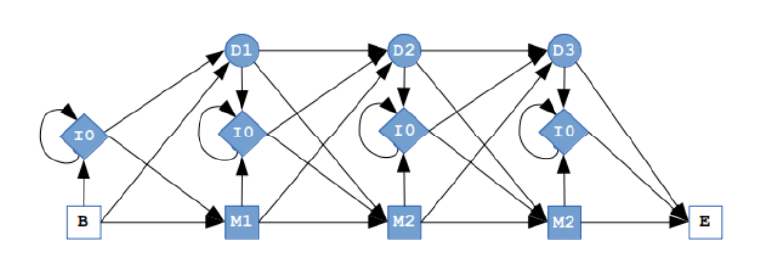
\includegraphics[width = 0.7\textwidth]{figs/general-hmm.png}
\caption{\textbf{Estructura general de un HMM de perfil.} Se muestra un HMM de perfil con 3 estados de coincidencia.}
\label{fig:gen-hmm}
\end{figure}

%21/10 - Luis del Peso
\section{Bases de datos de MSA}
Como ya se ha mencionado, una de las principales aplicaciones del MSA es la identificación de regiones conservadas (motivos y dominios) en secuencias relacionadas. A continuación, la región identificada puede representarse mediante una secuencia de consenso, un patrón, un PSSM o un HMM. Muchas regiones conservadas dentro de familias de proteínas han sido identificadas utilizando este protocolo y están depositadas en bases de datos específicas. Existen varias BD de este tipo, que difieren en cómo se codifican los motivos y cómo se construyeron. Estas BD pueden buscarse utilizando texto (es decir, una búsqueda por palabras clave) o utilizando una secuencia de consulta para encontrar motivos presentes en ella. Describiremos brevemente algunas de ellas:
\begin{itemize}
\item \textbf{Pfam:} La base de datos Pfam es una gran colección de motivos, dominios y familias de proteínas, cada uno de ellos representado por alineaciones de secuencias múltiples y modelos de Markov ocultos (HMM). Pfam consta de dos bases de datos. Pfam-A es una colección curada manualmente de familias de proteínas en forma de alineaciones de secuencias múltiples y perfiles HMM. Pfam-B es una base de datos derivada automáticamente de perfiles HMM.
\item \textbf{SMART:} Simple Modular Architecture Research Tool (SMART) es otra base de datos de familias de proteínas representadas como HMM de perfil.
\item \textbf{PROSITE:} Una base de datos de pequeños patrones en forma de expresiones regulares y reglas (expresiones regulares cortas que definen pequeños patrones de 4-5 residuos de longitud) y dominios en forma de perfiles PSSM. Todas estas expresiones se derivan manualmente del análisis de MSA y de la bibliografía. Un mismo motivo en una familia de proteínas puede definirse mediante un patrón, un perfil o ambos.
\end{itemize}

Existen recursos especializados que integran varias de las bases de datos individuales de familias de proteínas. El más popular es \href{https://www.ebi.ac.uk/interpro/}{InterPro} que, desde un único punto de entrada, permite un análisis exhaustivo de dominios y motivos proteicos.

\subsection{Búsqueda de motivos con InterPro [Ejercicio]}
Vamos a buscar los motivos y dominios de la proteína NP\_001023646 en InterPro. Tras evaluar la secuencia, se pueden observar 3 dominios descritos para la proteína en cuestión (figura \ref{fig:interpro}). Para cada dominio y motivo hay entradas en bases de datos distintas. 

\begin{figure}
\centering
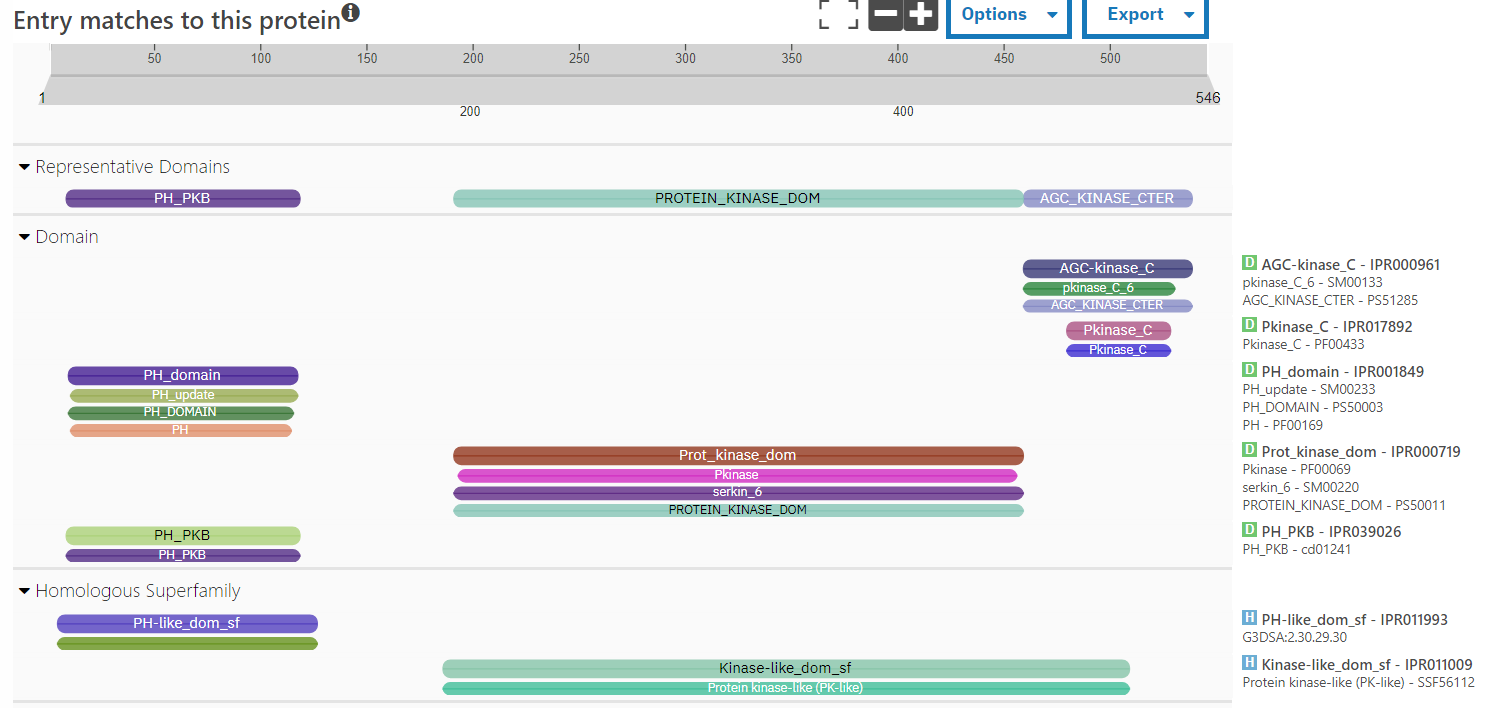
\includegraphics[width = \textwidth]{figs/interpro-ej.png}
\caption{Resultados de la búsqueda en Interpro de la proteína NP\_001023646.}
\label{fig:interpro}
\end{figure}

Desde la página de PFAM, se puede descargar los datos en crudo de HMM. En el fichero se encuentran los números de las distintas posiciones y tres filas para cada posición que representan respectivamente los valores de emisión en match y emisión en inserción para cada aminoácido definido en la parte superior y transición para cada estado mostrado debajo de los aminoácidos. En el caso de PROSITE, se muestra el patrón. 

\section{Búsqueda avanzada en bases de datos}
Los alineamientos de secuencias múltiples contienen mucha más información sobre una familia o dominio de proteínas que cualquier secuencia individual. Por tanto, si utilizamos como consulta una representación de un alineamiento en lugar de una secuencia individual, la búsqueda será mucho más sensible e identificará homólogos más distantes. Este es el enfoque utilizado por el Position-Specific Iterated BLAST o PSI-BLAST ($\Psi$-BLAST). Este BLAST especializado se inicia como un BLAST normal utilizando una consulta de proteínas para buscar en bases de datos de proteínas (figura \ref{fig:adv-blast}). A continuación, a partir de la lista de aciertos, selecciona aquellas proteínas que superan un determinado umbral de valor E y realiza un MSA de todas ellas junto con la consulta. A partir del MSA obtiene un PSSM y lo utiliza como consulta en una segunda iteración de búsqueda. A partir de los resultados de la segunda iteración selecciona nuevos aciertos encontrados y refina el PSSM para iniciar una tercera iteración. El proceso se repite varias veces hasta que no se encuentran nuevos aciertos (figura \ref{fig:adv-blast}).

\begin{figure}[htbp]
\centering
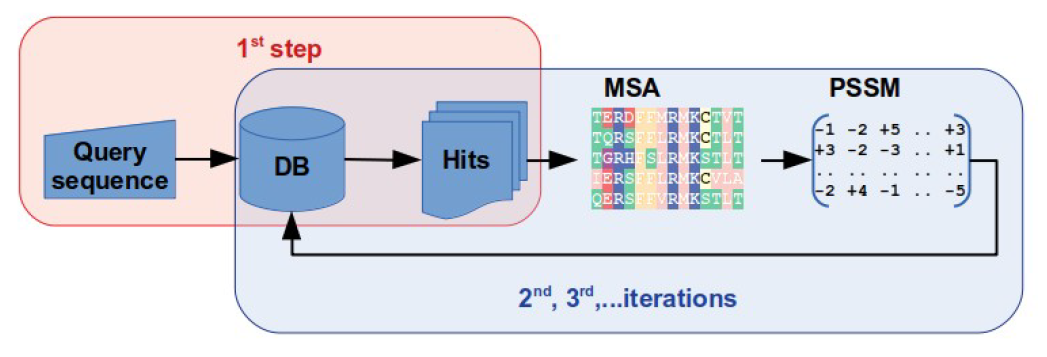
\includegraphics[width = \textwidth]{figs/advanced-blast.png}
\caption{\textbf{BLAST Iterado de Posición Específica}. La primera fase de PSI-BLAST es idéntica a la de una búsqueda BLAST normal. En la segunda fase, se seleccionan una serie de aciertos para producir un MSA y, a partir de él, un PSSM que se utiliza para buscar en la base de datos original. Esta segunda fase se repite tantas veces como sea necesario hasta que no se encuentren nuevos resultados significativos. Cada nueva iteración genera un nuevo PSSM a partir de los resultados de la búsqueda anterior.}
\label{fig:adv-blast}
\end{figure}

PSI-BLAST (y también PHI-BLAST, véase más adelante) generan PSSM que luego se utilizan para buscar en bases de datos, logrando una mayor sensibilidad que las búsquedas regulares basadas en secuencias. Los HMM de perfiles son modelos probabilísticos muy potentes que también pueden utilizarse para ayudar en la identificación de miembros distantes de una familia de proteínas. HMMER comprende un conjunto de programas que utilizan modelos de Markov ocultos de perfil para el análisis de secuencias. Uno de los programas, jackhmmer en HMMER, busca iterativamente una secuencia de proteínas en una base de datos de secuencias de proteínas. Conceptualmente es similar a PSIBLAST pero, internamente, genera un perfil HMM y lo utiliza para buscar en la base de datos (figura \ref{fig:hmmer}).

\begin{figure}[htbp]
\centering
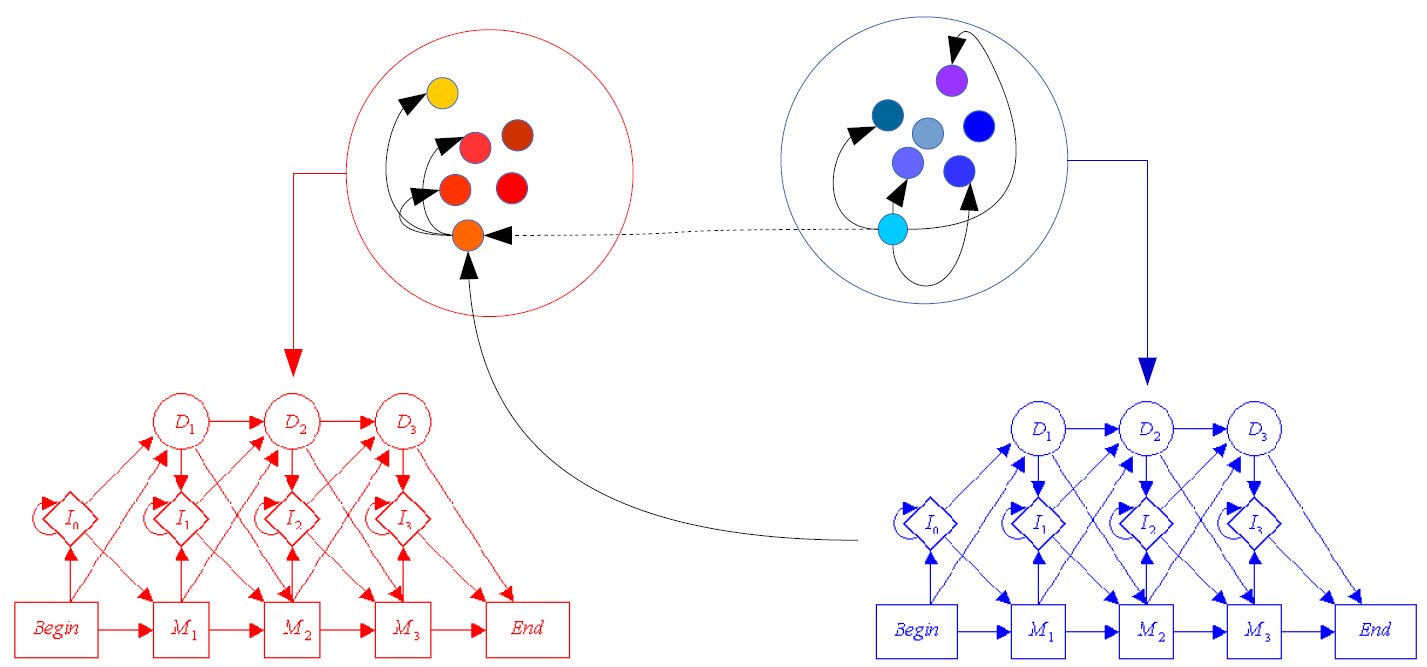
\includegraphics[width = \textwidth]{figs/hmmer.png}
\caption{Representación gráfica de HMMER.}
\label{fig:hmmer}
\end{figure}

Otro programa BLAST especializado es Pattern-Hit initiated BLAST o PHIBLAST($\Phi$-BLAST). Este programa es muy similar a PSI-BLAST, salvo que se inicia con una secuencia de consulta y un patrón (expresión regular), de forma que sólo se devuelven los resultados que coinciden con la consulta y contienen el patrón. A partir de los resultados de la primera búsqueda, el algoritmo genera un PSSM que se utiliza en las búsquedas posteriores.

\section{Técnicas de análisis de secuencias adicionales}
\subsection{Búsquedas de motivos}
Varios genes pueden compartir un sitio de unión de un mismo factor de transcripción. Sabiendo la secuencia de unión, se puede utilizar como patrón para buscar los match. En caso de tener una PSSM (por ejemplo, mediante ChIp-Seq) que represente el sitio de unión, se puede ir comparando la secuencia posición por posición con la PSSM y calcular la puntuación. Así, mediante ventanas deslizantes, se escanea toda la secuencia y encontrar todas las subsecuencias que sobrepasen un umbral y, por tanto, sean regiones de unión a ese factor de transcripción (figura \ref{fig:motif-location}). 

\begin{figure}[htbp]
\centering
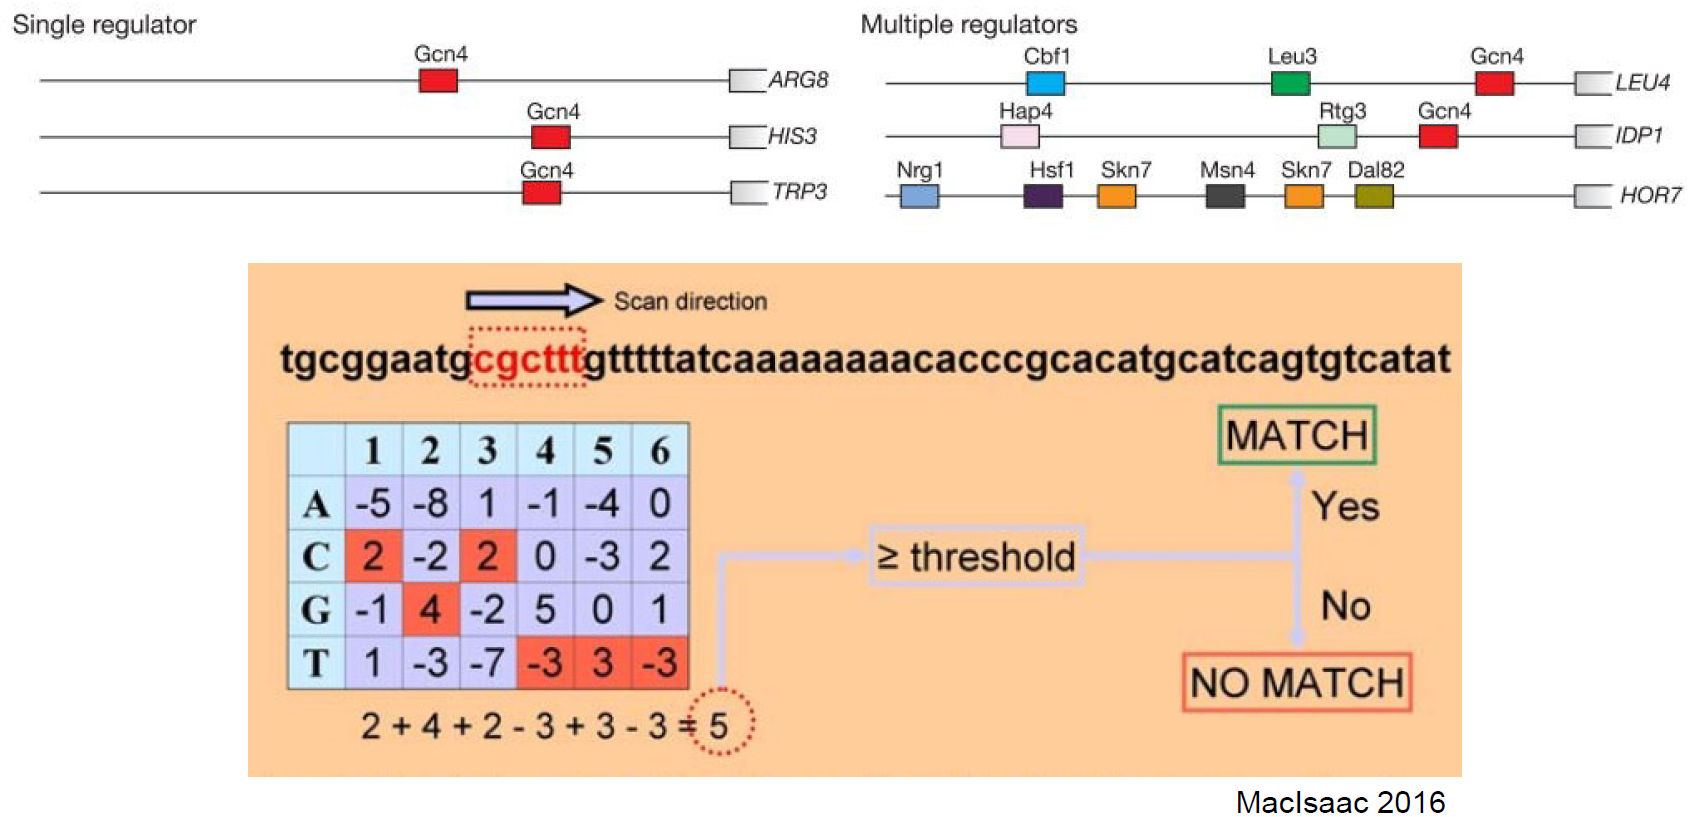
\includegraphics[width = \textwidth]{figs/motif-location.png}
\caption{Representación gráfica de una búsqueda de un motivo.}
\label{fig:motif-location}
\end{figure}

Recientemente se ha creado una base de datos de sitios de unión de factores de transcripción representados como PSSM y obtenidos mediante muchos métodos experimentales: \href{https://jaspar.genereg.net/}{Jaspar}. Además de las PSSMs, se podrían utilizar modelos ocultos de Markov. 

El problema de las PSSM es que son muy ruidosas y es fácil encontrar las secuencias por azar. Este ruido se puede restringir a las regiones de cromatina abierta. Otra forma que se utilizaba antes de tener esta información es mediante huellas filogenéticas. 

En la figura \ref{fig:conservation}, las regiones en color crema representan exones, los cuales tienen una alta presión de conservación. Fuera de las regiones exónicas, hay otras regiones que presentan una alta conservación, y que por tanto podrían representar enhancers. 

\begin{figure}[htbp]
\centering
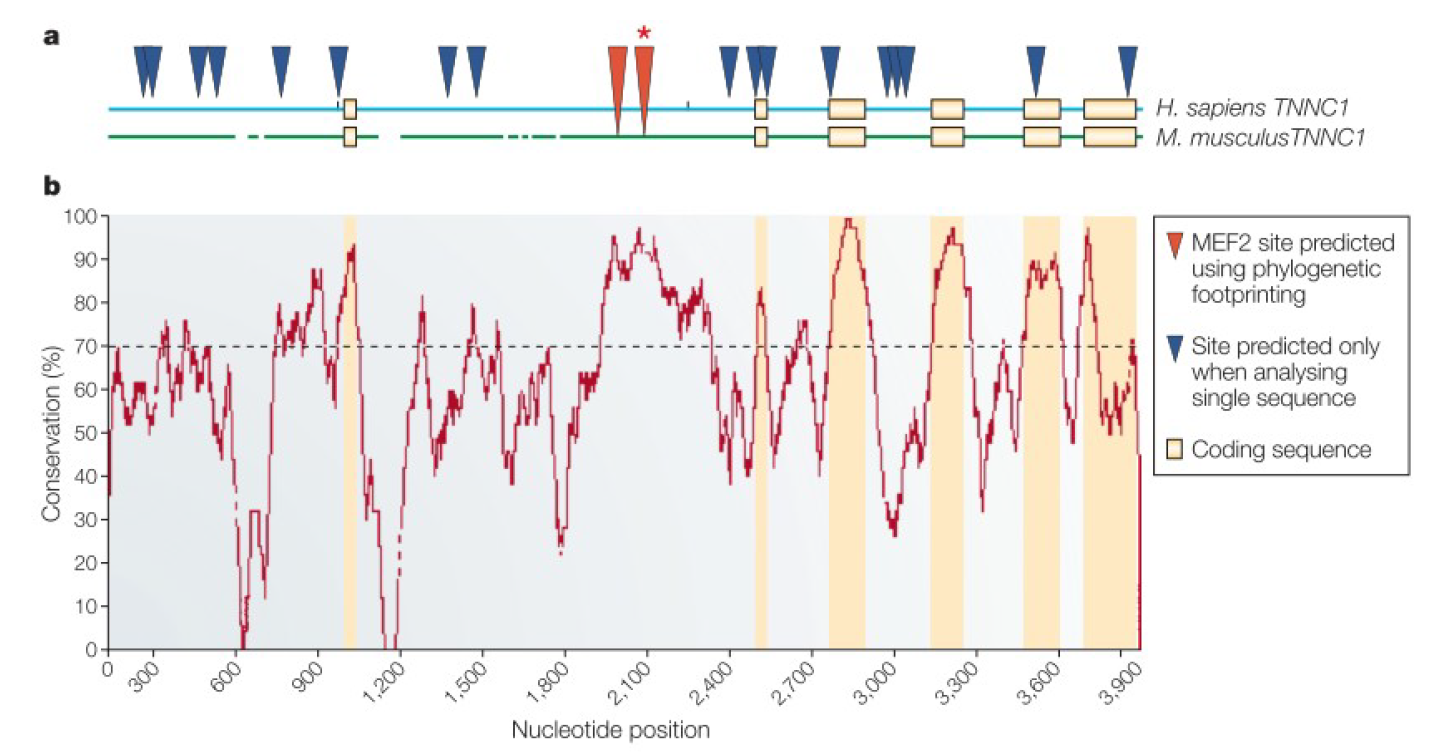
\includegraphics[width = 0.7\textwidth]{figs/noise-reduction.png}
\caption{Representación de regiones conservadas.}
\label{fig:conservation}
\end{figure}

%23/10 - Luis del Peso
\subsection{Enriquecimiento de motivos y análisis de asociación}
Esta idea se puede extender de la siguiente forma: Tenemos un conjunto de genes coexpresados en una situación concreta (por ejemplo, un tumor). Se extrae el ARN y se observan genes con una expresión similar en esa situación y en una control (no tumor, órgano sano) y genes con una expresión significativamente (estadísticamente) diferentes en ambas situaciones. Estos genes se denominan como genes expresados diferencialmente (DEG por sus siglas en inglés).
Dado este conjunto de genes, se quiere saber qué factor de transcripción los activa y causa esta expresión diferencial. Se toman genes DEG (mostrados en naranja) y genes no DEG como controles (mostrados en azul), y de ellos se toman los promotores o regiones reguladoras. A continuación se toma la lista de los factores de transcripción conocidos con sus matrices PSSM. De forma secuencial se toma cada factor de transcripción y se recorre cada una de las secuencias para ver si tiene sitio de unión para ese factor. Esto se realiza para todas las regiones reguladoras de DEG y no DEG y todos los factores de transcripción, generando una tabla como la observada en la figura \ref{fig:enrichment}. 
Finalmente se debe realizar un test de asociación como un test estadístico de Fisher o Chi cuadrado. 

\begin{figure}[htbp]
\centering
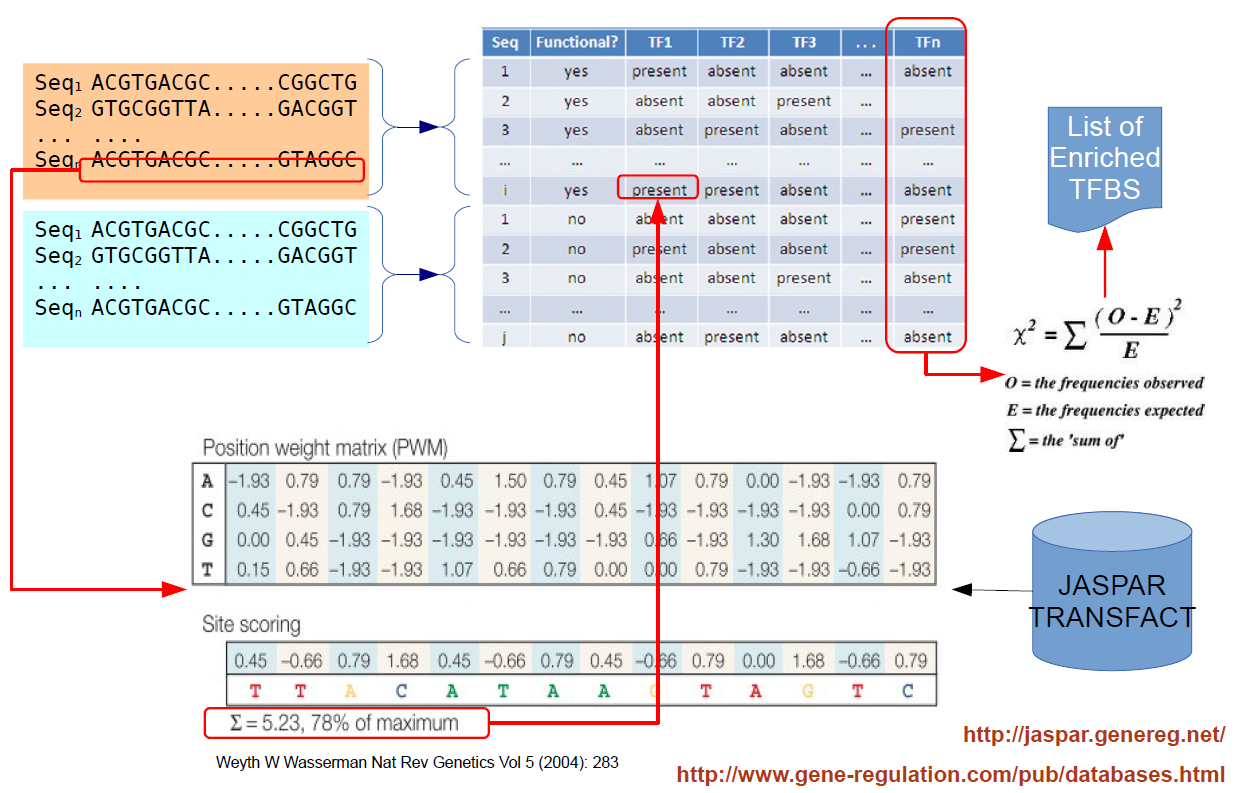
\includegraphics[width = 0.8\textwidth]{figs/motivos-enriquecidos.png}
\caption{Representación de motivos enriquecidos.}
\label{fig:enrichment}
\end{figure}

Para ver si hay una asociación entre las dos variables, se realiza un test de independencia para variables categóricas, que es un test de Fisher o de Chi cuadrado. Por ejemplo, al analizar DEG en tejidos tumoral y normal, se encuentran 258 de 11483 genes con una expresión mayor en el tumor que en el tejido sano. Mediante la búsqueda de motivos, se encuentra que el factor de transcripción HIF se une en 145 de los DEG y 3766 de los otros genes expresados. Con estos números, ¿la unión a HIF está significativamente enriquecida en DEG? Para ello, calculamos una tabla de contingencia:
\begin{table}[htbp]
\centering
\begin{tabular}{c | c c | c}
Observado & DEG & no DEG & \\ \hline
TFBS presente & 145 & 3766 & 3911 \\
TFBS no presente & 113 & 7459 & 7572 \\ \hline
& 258 & 11225 & 11483
\end{tabular}
\end{table}

Con estos números, ¿se puede concluir que existe una asociación entre ser DEG y tener un sitio de unión al factor de transcripción HIF? Utilizamos la fórmula del chi cuadrado:
$$ \chi^2 = \sum_{levels} \frac{(observado-esperado)^2}{esperado}$$

Una vez sabiendo el resultado, se compara el valor con la distribución de Chi cuadrado y se ve el área debajo de la curva por encima de ese valor (la probabilidad de que eso ocurra bajo la hipótesis nula, es decir, que no haya asociación). 

Para obtener los valores esperados, se debe mantener la proporción entre TFBS presentes y el total. Por ejemplo, para TFBS en DEG, se calcula:
$$\frac{3911}{11483} * 258 \approx 88$$
Así, la tabla completa queda de la siguiente forma:
\begin{table}[htbp]
\centering
\begin{tabular}{c | c c | c}
Esperado & DEG & no DEG & \\ \hline
TFBS presente & 88 & 3823 & 3911 \\
TFBS no presente & 170 & 7402 & 7572 \\ \hline
& 258 & 11225 & 11483
\end{tabular}
\end{table}

Tras calcular el Chi cuadrado, el resultado es significativo. Esto significa que hay una asociación a las variables, es decir, entre la unión del factor de transcripción y que los genes estén diferencialmente expresados. 

Esto sirve para un solo factor de transcripción, es decir, para una columna de la tabla mostrada en la figura \ref{fig:enrichment}. Para cada columna habrá que hacer una tabla de contingencia y un test estadístico, pero esto tiene un problema: en cada test estadístico se admite un error del 5\%, y al realizar múltiples test, se debe corregir para no encontrar tantos falsos positivos (con p valor significativo por azar). Así, se debe tomar el \textbf{p valor ajustado}, no en crudo. Además, se debe tener en cuenta el \textbf{tamaño de efecto} como segundo estadístico. Cuando el tamaño de muestreo es muy grande (por ejemplo, en los GWAS), el p valor suele ser muy pequeño, por lo que es importante saber cómo de diferente son las asociaciones. En el caso de tablas de contingencia, el tamaño del efecto suele ser el odds ratio:
$$Odds ratio = \frac{Odds_{TFBSpresente}}{Odds_{TFBSausente}}$$
$$\frac{\frac{145}{145+3766}/1-\frac{145}{145+3766}}{\frac{113}{113+7459}/1-\frac{113}{113+7459}} = \frac{0,0385}{0,0175} = 2,2$$

En este caso, el resultado es 2,2, lo que significa que hay dos veces más probabilidad de que el gen esté diferencialmente expresado si tiene sitio de unión de HIF que si no lo tiene. 

\subsection{Descubrimiento de motivos}
En los apartados anteriores, se trabajaba con factores de transcripción determinados experimentalmente y con matrices PSSM. Sin embargo, cuando un factor no se conoce, se puede identificar qué motivos tienen en común un conjunto de secuencias (por ejemplo, DEG) que no tienen otras secuencias (las secuencias control). El problema es que los factores de transcripción son algo promiscuos, uniéndose a unos motivos con una cierta flexibilidad. Hay algunos algoritmos que permiten solucionar este problema. Partiendo de las secuencias de interés (DEG), se empieza a buscar un motivo de X pares de bases. Se localizan los motivos en las distintas secuencias, viendo la secuencia y su localización. 

El \textbf{algoritmo EM (expectation-maximization)} coge un conjunto de secuencias y se inventa una matriz PSSM con la que rastrea las secuencias. Se identifica así las mejores posiciones de la secuencia, con las cuales se extraen los posibles motivos y se vuelve a construir la matriz para volver a rastrear las secuencias. Esta es una búsqueda heurística, por lo que se pueden obtener máximos locales. Por ello, se suelen repetir estas búsquedas para comparar los resultados e intentar aproximarse a los máximos globales.
\begin{figure}[htbp]
\centering
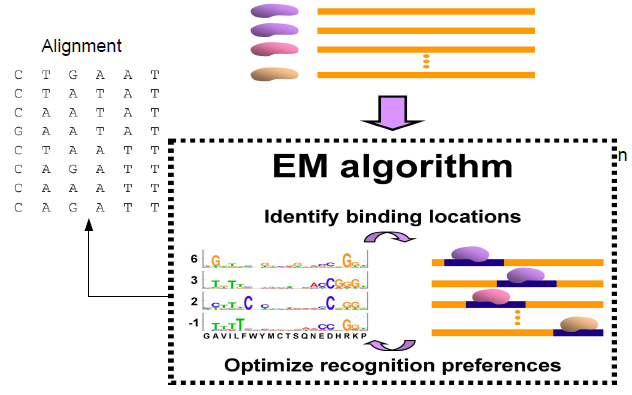
\includegraphics[width = 0.5\textwidth]{figs/algoritmo-em.png}
\caption{Esquema del algoritmo EM.}
\label{fig:em}
\end{figure}

Una simplificación del algoritmo se puede observar en la figura \ref{fig:em-simp}.
\begin{figure}[htbp]
\centering
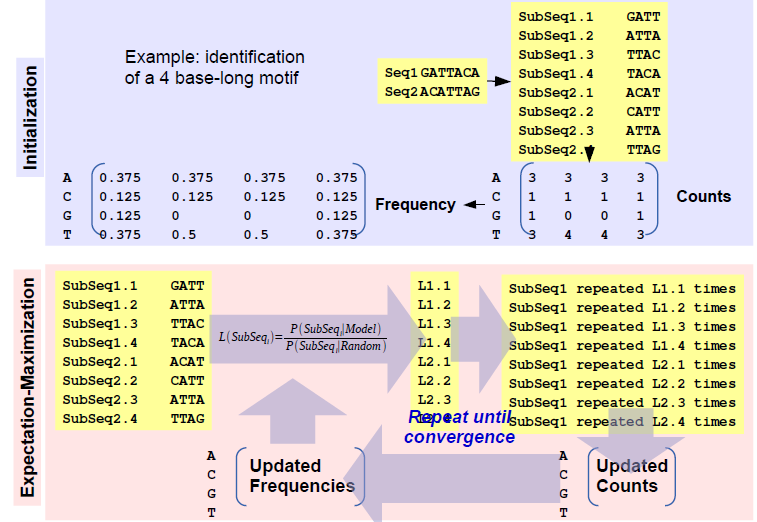
\includegraphics[width = 0.8\textwidth]{figs/em-pseudocode.png}
\caption{Simplificación del algoritmo EM. Durante la inicialización, se toman las subsecuencias de la longitud del motivo que se está buscando para las dos secuencias que se están analizando. Se cuentan las apariciones de cada nucleótido y se calculan las frecuencias. Para cada subsecuencia se calcula el score, y se repite la subsecuencia el número de veces que indique el score. Con ello, se vuelve a realizar el conteo de los nucleótidos, crear la matriz de frecuencias y se repite este proceso hasta la convergencia, es decir, cuando en uno de los pasos la matriz no cambie.}
\label{fig:em-simp}
\end{figure}

Normalmente, los factores de transcripción tienen entre 6 y 12 pares de bases. Por ello, en estos casos se inicia el algoritmo EM con 6 pares de bases, luego con 7, luego con 8, y así sucesivamente. Si el motivo tiene 8 pares de bases, se esperaría que el motivo encontrado en la búsqueda con 6 y 7 pares de bases esté contenido en el de 8. El resultado de todo esto es obtener la matriz PSSM para la cual realizar la búsqueda descrita en los puntos anteriores. 

\section{Quiz Moodle}
\subsection{Ejercicio 1}
Los retrovirus están asociados a una amplia variedad de cánceres en pollos, ratones, gatos y monos. Algunos retrovirus causan un tipo específico de cáncer poco después de la infección en una elevada proporción de animales, mientras que otros causan diversos cánceres tardíamente después de la infección en una proporción menor de animales.
Los retrovirus altamente oncogénicos son recombinantes de genes virales y del huésped. Los cánceres inducidos por estos virus vienen determinados por el gen transducido del huésped.
Los retrovirus que causan cáncer con una incidencia baja no contienen información insertada del huésped. Más bien, parecen causar cáncer a través de la alteración de la expresión de genes del huésped (celular) potencialmente oncogénicos.
El virus del sarcoma murino Harvey induce cáncer poco después de la infección y la proteína responsable de la transformación fue aislada y denominada «Transforming protein p29» (secuencia en el archivo «RASH\_MSVHA.fasta»). Una búsqueda blast contra la base de datos de proteínas completas reveló que el gen de mamífero más cercano es el protooncogen HRAS. Para identificar las diferencias entre estas proteínas que podrían explicar la capacidad transformante de la proteína viral, las alineas utilizando BLAST (utiliza las secuencias P01115, en el archivo «RASH\_MSVHA.fasta», y P01112 en el archivo «Ras\_superfam.fasta»). La proteína viral es \textbf{51 aminoácidos más larga} que la contraparte celular debido a una \textbf{fusión en la parte N-terminal} de la proteína. 

Entre las dos proteínas se encuentran 3 diferencias, pero no es viable ver cuál es la mutación oncogénica. Por ello, se realiza un MSA con toda la superfamilia Ras, incluyendo varios ortólogos y parálogos. Nos fijamos en los siguientes cambios, tomando al proteína RasH humana como índice: G12R (probable), A59T (probable), A122G (improbable) y Y71F (no hay cambio). Hay otros retrovirus que contienen oncogenes derivados de la proteína Ras, y realizando un MSA de ellos, nos fijamos en las mismas posiciones de antes: G12R (probable), A59T (improbable), A122G (improbable) y Y71F (no hay cambio). Por último, la proteína ERAS desempeña un papel importante en las propiedades de crecimiento tumoral de las células madre embrionarias. Repita el MSA de la superfamilia Ras incluyendo la secuencia de ERAS (la encontrará en el archivo «Ras\_active.fasta»). Compare el MSA de todos los miembros de la familia con o sin ERAS, cuál es el único residuo que se conserva en todos los miembros de la familia excepto ERAS50.

\subsection{Ejercicio 2}
Tenemos las siguientes frecuencias absolutas de nucleótidos en cada posición de un alineamiento:
\begin{table}[htbp]
\begin{tabular}{l | llllllllllllllllll}
A & 2  & 38 & 0  & 0  & 0  & 0  & 10 & 8  & 4  & 7  & 21 & 9  & 9  & 11 & 9  & 23 & 4  & 15 \\
C & 10 & 0  & 46 & 0  & 0  & 0  & 32 & 17 & 10 & 15 & 11 & 18 & 9  & 16 & 23 & 11 & 20 & 8  \\
G & 10 & 8  & 0  & 46 & 0  & 46 & 2  & 17 & 21 & 13 & 14 & 15 & 27 & 8  & 13 & 8  & 16 & 22 \\
T & 24 & 0  & 0  & 0  & 46 & 0  & 2  & 4  & 11 & 11 & 0  & 4  & 1  & 11 & 1  & 4  & 6  & 1 
\end{tabular}
\end{table}

Primero calculamos las frecuencias con pseudocuentas sumando 1 a todas las celdas:
\begin{table}[htbp]
\begin{tabular}{l | llllllllllllllllll}
A & 3  & 39 & 1  & 1  & 1  & 1  & 11 & 9  & 5  & 8  & 22 & 10 & 10 & 12 & 10 & 24 & 5  & 16 \\
C & 11 & 1  & 47 & 1  & 1  & 1  & 33 & 18 & 11 & 16 & 12 & 19 & 10 & 17 & 24 & 12 & 21 & 9  \\
G & 11 & 9  & 1  & 47 & 1  & 47 & 3  & 18 & 22 & 14 & 15 & 16 & 28 & 9  & 14 & 9  & 17 & 23 \\
T & 25 & 1  & 1  & 1  & 47 & 1  & 3  & 5  & 12 & 12 & 1  & 5  & 2  & 12 & 2  & 5  & 7  & 2 
\end{tabular}
\end{table} 

El siguiente paso es construir la tabla PWM con las frecuencias con pseudocuentas. Para ello, simplemente se toma el valor de cada celda y se divide por el sumatorio de los valores en esa posición: 
\begin{table}[htbp]
\begin{tabular}{l | llllllllllllllllll}
A & 0,06 & 0,78 & 0,02 & 0,02 & 0,02 & 0,02 & 0,22 & 0,18 & 0,1  \\
& 0,16 & 0,44 & 0,2  & 0,2  & 0,24 & 0,2  & 0,48 & 0,1  & 0,32 \\
C & 0,22 & 0,02 & 0,94 & 0,02 & 0,02 & 0,02 & 0,66 & 0,36 & 0,22 \\
& 0,32 & 0,24 & 0,38 & 0,2  & 0,34 & 0,48 & 0,24 & 0,42 & 0,18 \\
G & 0,22 & 0,18 & 0,02 & 0,94 & 0,02 & 0,94 & 0,06 & 0,36 & 0,44 \\
& 0,28 & 0,3  & 0,32 & 0,56 & 0,18 & 0,28 & 0,18 & 0,34 & 0,46 \\
T & 0,5  & 0,02 & 0,02 & 0,02 & 0,94 & 0,02 & 0,06 & 0,1  & 0,24 \\
& 0,24 & 0,02 & 0,1  & 0,04 & 0,24 & 0,04 & 0,1  & 0,14 & 0,04
\end{tabular}
\end{table}
\newpage
Con esa tabla, se calcula la PSSM. Para ello, se calcula $log_2(\frac{celda}{0,25})$:
\begin{table}[htbp]
\begin{tabular}{l | llllllllllllllllll}
A & -2,06 & 1,64  & -3,6 & -3,64 & -3,6 & -3,6 & -0,2 & -0,5 & -1,3 \\
& -0,6 & 0,82  & -0,32 & -0,32 & -0,1 & -0,32 & 0,94  & -1,32 & 0,36  \\
C & -0,18 & -3,64 & 1,91 & -3,64 & -3,6 & -3,6 & 1,4  & 0,53 & -0,2 \\
& 0,4  & -0,06 & 0,6   & -0,32 & 0,44 & 0,94  & -0,06 & 0,75  & -0,47 \\
G & -0,18 & -0,47 & -3,6 & 1,91  & -3,6 & 1,9  & -2,1 & 0,53 & 0,82 \\
& 0,2  & 0,26  & 0,36  & 1,16  & -0,5 & 0,16  & -0,47 & 0,44  & 0,88  \\
T & 1  & -3,64 & -3,6 & -3,64 & 1,91 & -3,6 & -2,1 & -1,3 & -0,1 \\
& -0,1 & -3,64 & -1,32 & -2,64 & -0,1 & -2,64 & -1,32 & -0,84 & -2,64
\end{tabular}
\end{table}

El siguiente paso es calcular la entropía de Shannon y la información. Previamente necesitamos la tabla PWM sin pseudocuentas, que sería la siguiente:

\begin{table}[h]
\begin{tabular}{l | llllllllllllllllll}
A & 0,04 & 0,83 & 0 & 0 & 0 & 0 & 0,22 & 0,17 & 0,09 \\
& 0,2 & 0,46 & 0,2  & 0,2  & 0,24 & 0,2  & 0,5  & 0,09 & 0,33 \\
C & 0,22  & 0    & 1 & 0 & 0 & 0 & 0,7  & 0,37 & 0,22 \\
& 0,3 & 0,24 & 0,39 & 0,2  & 0,35 & 0,5  & 0,24 & 0,43 & 0,17 \\
G & 0,22  & 0,17 & 0 & 1 & 0 & 1 & 0,04 & 0,37 & 0,46 \\
& 0,3 & 0,3  & 0,33 & 0,59 & 0,17 & 0,28 & 0,17 & 0,35 & 0,48 \\
T & 0,52 & 0    & 0 & 0 & 1 & 0 & 0,04 & 0,09 & 0,24 \\
& 0,2 & 0    & 0,09 & 0,02 & 0,24 & 0,02 & 0,09 & 0,13 & 0,02
\end{tabular}
\end{table}

La entropía de Shannon se calcula para cada posición. Se sigue la siguiente fórmula: $- \sum (probabilidad) \cdot log_2 (probabilidad) $. Cuando la probabilidad es 0, se considera que el logaritmo también lo es. Los valores resultantes son los siguientes:

1,64 - 0,67 - 0 - 0 - 0 - 0 - 1,24 - 1,81 - 1,8 - 1,9 - 1,53 - 1,82 - 1,49 - 1,96 - 1,6 - 1,74 - 1,74 - 1,6


Por último, es necesario calcular la información. La entropía máxima para cada posición es de 2, por lo que hay que restarle la entropía de Shannon. Así, la información para cada posición es la siguiente: 

0,36 - 1,33 - 2 - 2 - 2 - 2 - 0,76 - 0,19 - 0,2 - 0,1 - 0,47 - 0,18 - 0,51 - 0,04 - 0,4 - 0,26 - 0,26 - 0,4


\subsection{Ejercicio 3}
Contamos con las siguientes frecuencias relativas:
\begin{table}[h]
\centering
\begin{tabular}{l | llllll}
A & 0,68 & 0,11 & 0,02 & 0,86 & 0,16 & 0,41 \\
C & 0,08 & 0,04 & 0,01 & 0,03 & 0,05 & 0,11 \\
G & 0,08 & 0,8  & 0,96 & 0,04 & 0,67 & 0,24 \\
T & 0,16 & 0,05 & 0,01 & 0,07 & 0,12 & 0,24
\end{tabular}
\end{table}

Queremos dibujar un logo, por lo que debemos calcular la información para cada posición y la altura de cada letra en cada posición. La información se calcula como entropía anterior - entropía posterior. La entropía anterior es 2, y la entropía posterior se calcula como $- \sum (nucleotido) \cdot log_2 (nucleotido)$ para cada posición. Una vez sabiendo la información, para la altura de cada nucleótido se multiplica la altura total de la columna por la frecuencia de cada nucleótido. La tabla resultante es la siguiente:
\begin{table}[htbp]
\centering
\begin{tabular}{l | llllll}
Info (column height) & 0,62 & 0,99 & 1,70 & 1,21 & 0,61 & 0,13 \\
A height & 0,42 & 0,11 & 0,03 & 1,04 & 0,10 & 0,05 \\
C height & 0,05 & 0,04 & 0,02 & 0,04 & 0,03 & 0,01 \\
G height & 0,05 & 0,79 & 1,63  & 0,05 & 0,41 & 0,03 \\
T height & 0,10  & 0,05 & 0,012 & 0,08 & 0,07 & 0,03
\end{tabular}
\end{table}

Por último, hay que indicar la posición del nucleótido A para cada posición en el logo. Las posiciones de los distintos residuos se determinan por la frecuencia, siendo los nucleótidos más frecuentes los que se encuentran en primera posición (más arriba). Por tanto, fijándonos en la frecuencia de A en comparación con la de los demás nucleótidos para cada posición de la secuencia, su posición en el logo será la siguiente: 1 2 2 1 2 1.

\subsection{Ejercicio 4}
Tenemos el siguiente MSA con su representación de un perfil HMM.
\begin{figure}[htbp]
\centering
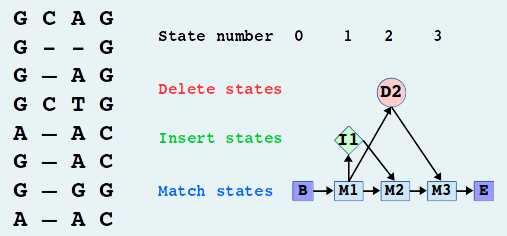
\includegraphics[width = 0.5\textwidth]{figs/moodle-msa-ej4.png}
\end{figure}

A partir de este modelo, primero calculamos la matriz de emisión de match. Para ello, calculamos en cada posición match el número de veces que aparece el nucleótido en cuestión y se divide por la cantidad de secuencias que tienen match en esa posición. Por ejemplo, en la posición match 1, A aparece 2 de 8 veces, por lo que su emisión es $2/8 = 0,25$. En la posición match 2, A aparece 5 veces, pero solo 7 secuencias tienen un match en esa posición (la otra secuencia tiene un gap), por lo que en este caso su emisión sería $5/7 = 0,71$. Así, la tabla resuelta sería la siguiente:
\begin{table}[htbp]
\centering
\begin{tabular}{l | l l l l l}
& B & 1 & 2 & 3 & E \\ \hline
A & - & 0,25 & 0,71 & 0 & - \\
C & - & 0 & 0 & 0,375 & - \\
G & - & 0,75 & 0,14 & 0,625 & - \\
T & - & 0 & 0,14 & 0 & - 
\end{tabular}
\end{table}

La matriz de emisión para las inserciones utiliza la misma lógica, pero centrándose en las inserciones. En este caso, sólo hay una posición de inserción después del match 1, y solo está presente en dos secuencias. Como las dos secuencias tienen una C como inserción, el estado de emisión de inserción para C es $2/2 = 1$.
\begin{table}[htbp]
\centering
\begin{tabular}{l | l l l l l}
& B & 1 & 2 & 3 & E \\ \hline
A & 0 & 0 & 0 & 0 & - \\
C & 0& 1 & 0 & 0 & - \\
G & 0 & 0 & 0& 0 & - \\
T & 0& 0 & 0 & 0 & - 
\end{tabular}
\end{table}

Por último queda calcular la matriz con las probabilidades de transición. Esta matriz se divide en tres: la transición desde match, desde inserción y desde delete. La suma de los valores para cada uno debe dar 1 o 0 para cada posición. Al igual que en los casos anteriores, contamos las ocurrencias del evento que se produce (si de match pasa a match, si de match pasa a delete, etc) del total de ocurrencias. Por ejemplo, las 8 secuencias comienzan en match, por lo que la probabilidad de M-M en B (begin) es de $8/8 = 1$. Sin embargo, desde la posición 1, solo 5 secuencias pasan a match; dos pasan a insert y una a delete. Por ello, M-M equivale a $5/8 = 0,625$, M-I a $2/8 = 0,25$ y M-D a $1/8 = 0,125$. Así, la tabla completa queda de la siguiente forma:
\begin{table}[htbp]
\centering
\begin{tabular}{l | l l l l l}
& B & 1 & 2 & 3  \\ \hline
M-M & 1 & 0,625 & 1 & 1 \\
M-D & 0 & 0,125 & 0 & - \\
M-I & 0 & 0,25 & 0 & 0 \\ \hline
I-M & 0& 1 & 0 & 0 \\
I-D & 0 & 0 & 0 & - \\
I-I & 0 & 0 & 0 & 0 \\ \hline
D-M & - & 0 & 1 & 0 \\
D-D & - & 0 & 0 & - \\
D-I & - & 0 & 0 & 0
\end{tabular}
\end{table}